\documentclass{standalone}

\begin{document}

\section[SymptomsNet]{SymptomsNet}\label{chimera:symptomsnet}

Finding relationships between symptoms and diseases and their reflections on system-wise perspectives such as genomics and metabolomics, thus remains a crucial issue for medical research but nonetheless an open one mainly due to the complexity and the heterogeneity of the available data.
The relation between symptoms and diseases can be used to see analogies and co-occurrences of different pathology, including morbidity and co-morbidity.
The construction of a unique and consistent database of these kind of data is an open problem for the research and a crucial task for many actual projects.
The main problems arise from the complexity and heterogeneity of the available data and from the many nomenclatures used by different public databases.
In fact, in many cases it is not so clear how to infer about the association between symptoms and diseases, and, in addition, different data sources provide different relations.
These information are provided as sentences and periods, of variable length and we have to face on the problem of the different synonyms and periphrases used to describe the same concept.

In our work we used large-scale public on-line databases to construct a bipartite network of human symptoms-diseases.
We used common tools of natural language processing to clean and uniform the data to maximize the overlap between the different sources.
After its construction, this network is used to establish a score for the different words based on the centrality measure of the node.

This complex map of association can further be used to connect other data sources and enrich the diseases description from other medical points of view.

Many on-line databases offer auto-diagnosis tools and search engine in which insert a list of symptoms or diseases and obtain the corresponding \quotes{diagnoses}.
While many international databases are quite consistent and provided by medical/biological research groups, the available data in Italian language are quite scarce.

Using the Italian version of public \emph{on-line doctor} websites we can obtained the needed informations.
We applied a set custom web scraping pipelines\footnote{
  We would stress that the extremely variety of the websites requires an equally varied set of web-scraping algorithms.
  Thus for each web page taken into account an appropriated web-scraper was developed.
} to the different web pages to extract the medical informations and we mainly focused on sites which highlight the relationship between symptoms and diseases.
As discussed above the Italian data sources are quite fewer than the English ones so only three web pages were involved into our analysis: \href{https://m.my-personaltrainer.it/}{My PersonalTrainer}, \href{http://www.sanihelp.it/}{SaniHelp} and \href{http://www.sapere.it/}{Sapere.it}.
All these three sites provide an organized series of tables which associate a disease to the corresponding symptoms.
These databases are certainly not robust from a scientific point-of-view and their vulnerability is shown also by a non-rigid labeling of the two classes: in multiple cases we can find a disease as symptom of an other one and in many cases there is not a perfect agreement between the three data sources.
However, we can ensure that the most part of symptoms-disease association was validated by \quotes{authoritative} agencies in our databases selection.

The data extracted from the three websites cover a wide range of possible diseases and from each of them we obtained a network with a size of few thousand of nodes, our \textsf{SymptomsNet}.
The overlap of the single words contained in the \quotes{disease-sentences} is quite low so a robust pre-processing was needed.
The nodes were processed by standard natural language processing techniques and from each name the word stem was extracted to maximize the merging between the different sources.
If two diseases show different symptoms we decided to concatenate the list of edges to not lose information.

The processing outputs generated a network with 2285 nodes and more than 29k links (only the 1\% of the total number of possible links).
The final \textsf{SymptomsNet} obtained by the merging of the three database sources is reported in Figure\ref{fig:net} in which the size of nodes is proportional to the degree (Tab.\ref{tab:rank} for the top ranking links).

\begin{figure}[htbp]
\centering
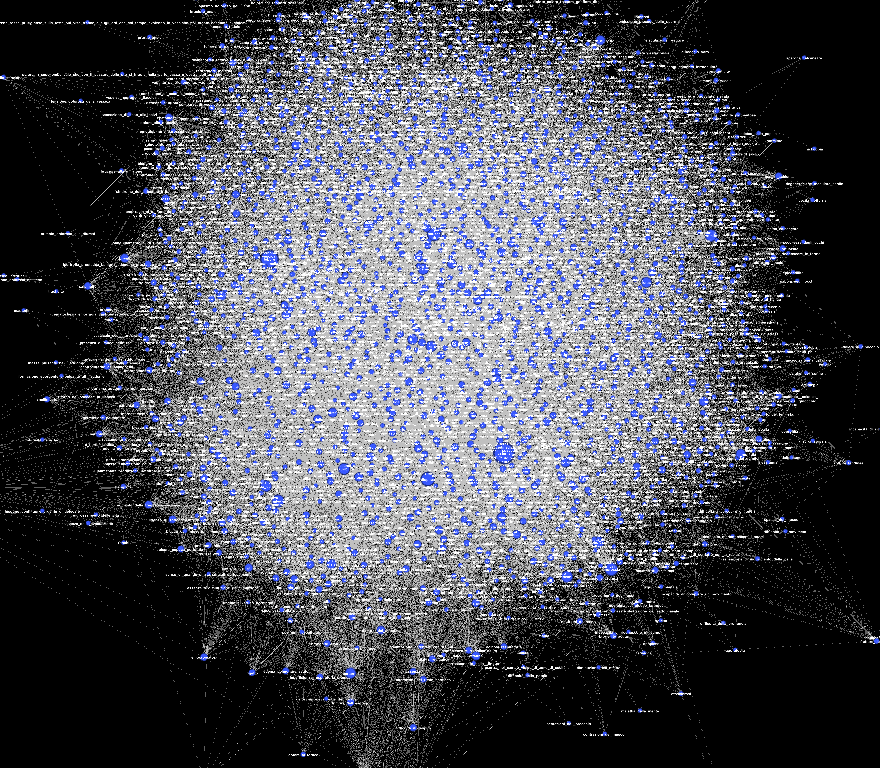
\includegraphics[width=.8\linewidth]{symnet.png}
\caption{Symptoms-disease network generated by the merging of three public Italian web-pages of auto-diagnosis search engine.
The network connects symptom and disease words according to validation agencies.
The network comprise 2285 nodes and more than 29k links.
In the figure the node size is proportional to its centrality (degree score).
In this way the most common symptoms/diseases represent the biggest nodes.
}
\label{fig:net}
\end{figure}

\begin{table}[htbp]
\centering
\begin{tabular}{lccc}
\hline \rowcolor{darkgrayrow}
Disease/Symptom & degree \\
\hline
Astenia         & 384    \\
Febbre          & 313    \\
Dispnea         & 225    \\
Nausea          & 222    \\
Anoressia       & 201    \\
Ematemesi       & 193    \\
Vomito          & 182    \\
Debolezza       & 176    \\
Affaticamento   & 176    \\
Esaurimento     & 172    \\
Mancanza Forze  & 168    \\
Edema           & 158    \\
\hline
\end{tabular}
\caption{Top ranking link in the Symptos-Diseases network. Also in this case we can notice \quotes{periphrases/synonyms} associated to the same symptom as \emph{Debolezza} and \emph{Mancanza Forze}}.
\label{tab:rank}
\end{table}

In this simple example we can already notice as the most central (big) nodes are associated to most common symptoms-diseases, as expected.
This result can be already interpreted as a validation of the performed processing.
There are however some conceptual repetitions into the node list: if it could be a problem for the use of this network structure for theoretical analyses, it is a strength for our application to the FiloBlu project.
In fact, this kind of occurrences allow us to consider a wide range of possible synonyms in the scorer attribution and so they can enforce the synthetic text generation.

We can conclude that from this very simple and preliminary work we are able to propose a novel symptoms-disease network based on Italian public databases and far as the author knows no other equivalent results are reported in literature.
This works allowed also the realization of a novel database obtained by the union of the most common available data.
The centrality measures extracted by this network can be used as floating point scorers or weight for the corresponding word
in the diseases association and despite the still there issues it could be consider a valid input for a toy-model text generator.

This results encourage us in the usage of this kind of techniques for further and deeper applications and these ideas brought us to the development of the \textsf{CHIMeRA} project.
If the above results could be reasonably good for the FiloBlu project purposes we could perform better using English data sources and with a better tuning of our natural language processing pipeline.
In the next section we will discuss about what natural language processing means in the modern researches and we will describe the pipeline and databases using into the \textsf{CHIMeRA} project.

\end{document}
